\documentclass{article}

\usepackage{fancyhdr}
\usepackage{graphicx}

\pagestyle{fancy}
\lhead{Alex Taylor}
\cfoot{}
\rfoot{\thepage}

\title{Database Design}
\author{Alex Taylor - amt22@aber.ac.uk}

\begin{document}

\maketitle
\begin{center}
	Version 1.0 (Release)
\end{center}
\tableofcontents
\thispagestyle{empty}
\newpage

\section{Tables}
There will be six tables:
\begin{enumerate}
	\item Admins
	\item Admin\_Details
	\item Quizzes
	\item Questions
	\item Quizzes\_Questions
	\item Sessions
\end{enumerate}

The first two store information about the Admin users, i.e. the lecturers, the Admin table being used to store the name, email and other details, whilst the Admin\_Details table will be for storing password and login details.

Quizzes will store the name of a quiz and the id of the admin who created it. The Questions table stores all the questions created and the Quizzes-Questions table is the link between the two. It stores which questions belong to which quiz.

\section{Entity Relationship Diagram}
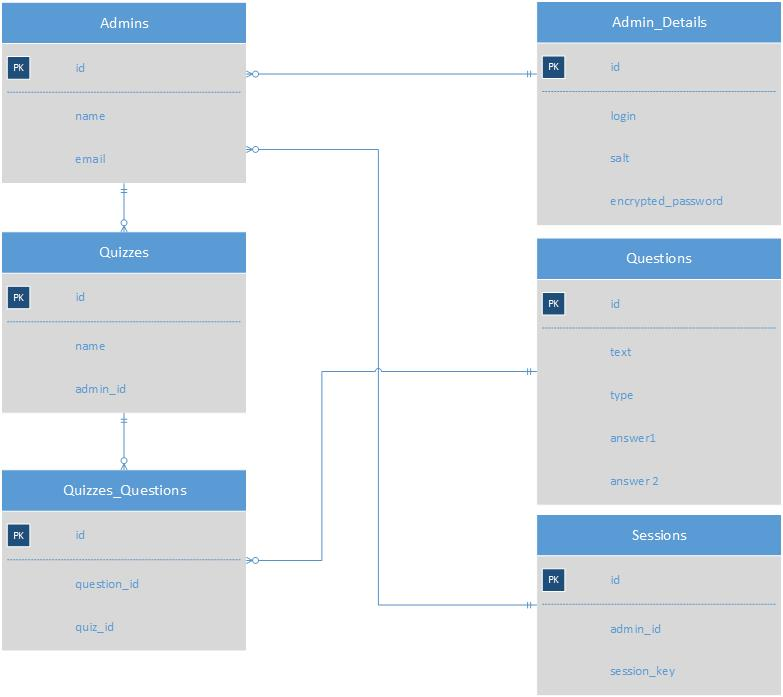
\includegraphics[width=\textwidth]{ERDiagram}

\end{document}